\documentclass[12pt, a4paper]{article}
\usepackage{xcolor}
\usepackage[top=2cm, bottom=2cm, left=2.0cm, right=2.0cm]{geometry}
\geometry{a4paper}
\usepackage{tikz}
\usetikzlibrary{trees, positioning, shapes, arrows.meta, shapes.geometric}
\usepackage{forest}
\usepackage{amsmath}
\usepackage{algorithm}
\usepackage{algpseudocode}

\begin{document}

\title{Monte Carlo Tree Search (MCTS)}
\author{Christophe Louargant}
\date{\today}
\maketitle

\begin{abstract}
This document provides a comprehensive visualization of Monte Carlo Tree Search
algorithms for the two-player HEX game.
\end{abstract}

\section*{Introduction to Monte Carlo Tree Search}

Monte Carlo Tree Search (MCTS) is a heuristic search algorithm that
combines the precision of tree search with the generality of random sampling.
Unlike traditional minimax algorithms that require evaluation functions,
MCTS uses random playouts to estimate the value of positions.\\
In MCTS a game is represented by a \textbf{game tree} which is a tree
in which every node represents a state of the game. The very root of the
tree represent the initial state of the game (before any move\footnote{
    a move is a transition from a node to one of its children
} is done).
After choosing a move you end up in a child node. This child node is
a root node for its subtree. Since for HEX game there is no point remembering
the path leading to the current state, we can consider the tree starting from
the new state of the game.

\section*{The Core MCTS Algorithm}

The four-phase structure repeated for many iterations:

\begin{enumerate}
    \item \textbf{Selection}: Traverse the tree from root to leaf using UCB1
    \item \textbf{Expansion}: Add new child node when reaching a leaf
    \item \textbf{Simulation}\footnote{
        Sometimes goes by the names \it{rollout}, \it{playout}, and \it{sampling}.}:
        Run random playout from the new node.
    \item \textbf{Backpropagation}\footnote{
        Sometimes called \it{backup}.}:
        Update statistics along the path
\end{enumerate}

\section*{UCB1\footnote{UCB1 applied to trees is essentially UCT
(Upper Confidence bounds applied to Trees)} Formula: The Bandit Component}

\[
\text{UCB1}(i) = \frac{w_i}{n_i} + c \sqrt{\frac{\ln N}{n_i}}
\]

Where:
\begin{itemize}
    \item $w_i$: Number of wins for node $i$
    \item $n_i$: Number of visits for node $i$  
    \item $N$: Total number of visits to parent node
    \item $c$: Exploration constant (typically $\sqrt{2}$)
\end{itemize}

\section*{Naive MCTS}

In Naive MCTS, we make a critical assumption:
\textbf{the opponent plays randomly}.
This assumption simplifies the problem significantly:

\begin{itemize}
    \item \textbf{No opponent modeling}: We don't need to consider the opponent's optimal responses
    \item \textbf{Immediate evaluation}: After our move, the outcome depends only on random play
    \item \textbf{Computational efficiency}: Much faster than building deep trees
\end{itemize}

Since we assume random opposition, there's no benefit to looking deeper than our immediate move. The random playout from depth 1 already gives us a statistically meaningful evaluation of each move's quality.

\subsection*{Step-by-Step Visualization}

\subsubsection*{Current State}
Since there is no point keeping the path from the initial state (empty board)
to current state, the tree that the algorithm build has a maximum depth of 1
with the root representing the current state of the game.

Let's consider that it is the turn of player 1 (\textcolor{blue}{Blue} player)
to play and that it has to choose between 5 free positions.

The root node of the tree represent the board current state and it has
5 children (5 available moves: $A_1, A_2, A_3, A_4, A_5$. All unvisited).

\caption{A simple MCTS tree visualization.}
\label{fig:naive_mcts}
\end{figure}

\begin{center}
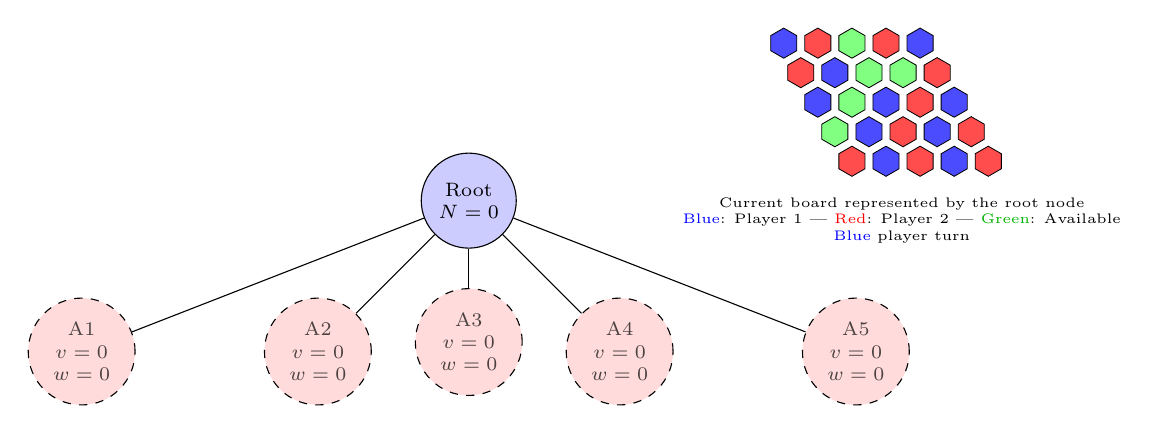
\begin{tikzpicture}[
    node distance=2.35cm,
    treenode/.style={circle, draw, minimum size=1cm, align=center, font=\scriptsize},
    root/.style={treenode, fill=blue!20, font=\scriptsize},
    unvisited/.style={treenode, fill=red!20, fill opacity=0.7, draw, dashed},
    visited/.style={treenode, fill=green!20},
    simulation/.style={rectangle, draw, dashed, fill=yellow!20},
    % Hex board styles
    hexagon/.style={
        regular polygon,
        regular polygon sides=6,
        minimum size=0.33cm,
        draw=black,
        line width=0.3pt,
        rotate=90
    },
    player1/.style={hexagon, fill=blue!70},
    player2/.style={hexagon, fill=red!70},
    available/.style={hexagon, fill=green!50}
]

% Root node
\node[root] (root) {Root\\$N=0$};

% Available moves (unvisited)
\node[unvisited, below left=1cm and 4cm of root] (a1) {A1 \\ $v=0$ \\ $w=0$};
\node[unvisited, below left=1cm and 1cm of root] (a2) {A2 \\ $v=0$ \\ $w=0$};
\node[unvisited, below=0.5cm of root] (a3) {A3 \\ $v=0$ \\ $w=0$};
\node[unvisited, below right=1cm and 1cm of root] (a4) {A4 \\ $v=0$ \\ $w=0$};
\node[unvisited, below right=1cm and 4cm of root] (a5) {A5 \\ $v=0$ \\ $w=0$};

% Edges
\draw (root) -- (a1);
\draw (root) -- (a2);
\draw (root) -- (a3);
\draw (root) -- (a4);
\draw (root) -- (a5);

% Hex board positioning (to the right of root)
\begin{scope}[shift={(4,0.5)}, scale=0.5]
% Define hex grid parameters
\def\hexwidth{0.866}  % sqrt(3)/2
\def\hexheight{0.75}  % 3/4 of the hexagon height

% Draw 5x5 hex board
% Row 1 (top)
\node at (0*\hexwidth, 4*\hexheight) [player1] {};
\node at (1*\hexwidth, 4*\hexheight) [player2] {};
\node at (2*\hexwidth, 4*\hexheight) [available] {};
\node at (3*\hexwidth, 4*\hexheight) [player2] {};
\node at (4*\hexwidth, 4*\hexheight) [player1] {};

% Row 2
\node at (0.5*\hexwidth, 3*\hexheight) [player2] {};
\node at (1.5*\hexwidth, 3*\hexheight) [player1] {};
\node at (2.5*\hexwidth, 3*\hexheight) [available] {};
\node at (3.5*\hexwidth, 3*\hexheight) [available] {};
\node at (4.5*\hexwidth, 3*\hexheight) [player2] {};

% Row 3 (middle)
\node at (1*\hexwidth, 2*\hexheight) [player1] {};
\node at (2*\hexwidth, 2*\hexheight) [available] {};
\node at (3*\hexwidth, 2*\hexheight) [player1] {};
\node at (4*\hexwidth, 2*\hexheight) [player2] {};
\node at (5*\hexwidth, 2*\hexheight) [player1] {};

% Row 4
\node at (1.5*\hexwidth, 1*\hexheight) [available] {};
\node at (2.5*\hexwidth, 1*\hexheight) [player1] {};
\node at (3.5*\hexwidth, 1*\hexheight) [player2] {};
\node at (4.5*\hexwidth, 1*\hexheight) [player1] {};
\node at (5.5*\hexwidth, 1*\hexheight) [player2] {};

% Row 5 (bottom)
\node at (2*\hexwidth, 0*\hexheight) [player2] {};
\node at (3*\hexwidth, 0*\hexheight) [player1] {};
\node at (4*\hexwidth, 0*\hexheight) [player2] {};
\node at (5*\hexwidth, 0*\hexheight) [player1] {};
\node at (6*\hexwidth, 0*\hexheight) [player2] {};

% Small legend
\node at (3, -1.5) [font=\tiny, align=center] {
    Current board represented by the root node \\
    \textcolor{blue}{Blue}: Player 1 | \textcolor{red}{Red}: Player 2 | \textcolor{green!70!black}{Green}: Available \\
    \textcolor{blue}{Blue} player turn
};
\end{scope}

\end{tikzpicture}
\end{center}

\subsubsection*{Iteration 1: First Expansion}

All nodes have UCB1 = $\infty$ (division by zero). Randomly select A1.

% \begin{center}
% \begin{tikzpicture}[
%     node distance=2.35cm,
%     treenode/.style={circle, draw, minimum size=1cm, align=center, font=\scriptsize},
%     root/.style={treenode, fill=blue!20, font=\scriptsize},
%     unvisited/.style={treenode, fill=red!20, fill opacity=0.7, draw, dashed},
%     selected/.style={treenode, fill=red!20},
%     visited/.style={treenode, fill=green!20},
%     simulation/.style={rectangle, draw, dashed, fill=yellow!20, align=center}
% ]

% % Root node
% \node[root] (root) {Root \\ $N=0$};

% % A1 is being expanded (selected)
% \node[selected, below left=1cm and 4cm of root] (a1) {A1 \\ $v=0$ \\ $w=0$};
% \node[unvisited, below left=1cm and 1cm of root] (a2) {A2 \\ $v=0$ \\ $w=0$};
% \node[unvisited, below=0.5cm of root] (a3) {A3 \\ $v=0$ \\ $w=0$};
% \node[unvisited, below right=1cm and 1cm of root] (a4) {A4 \\ $v=0$ \\ $w=0$};
% \node[unvisited, below right=1cm and 4cm of root] (a5) {A5 \\ $v=0$ \\ $w=0$};

% % Simulation cluster
% \node[simulation, below=2cm of a1] (sim1) {Simulation \\ Result: Win};

% % Edges and annotations
% \draw[->, thick, red] (root) -- node[above, sloped] {Selected} (a1);
% \draw (root) -- (a2);
% \draw (root) -- (a3);
% \draw (root) -- (a4);
% \draw (root) -- (a5);
% \draw[dashed, ->] (a1) -- (sim1);

% \end{tikzpicture}
% \end{center}

\begin{center}
\begin{forest}
    for tree={align=center, font=\scriptsize,s sep=1cm,
    l sep=1.5cm,edge={-Stealth, thin, draw=black!70},circle,
    draw=black!70, dashed, minimum size=1.5cm, inner sep=0pt,},
    root/.style={fill=blue!20, solid, edge={solid, draw=black}},
    unvisited/.style={fill=red!20, fill opacity=0.7, draw, dashed},
    selected/.style={fill=red!20, solid, draw=red,
    line width=0.8pt, edge={-Stealth, thick, red, solid},
    edge label={node[midway, above, font=\small, text=red, sloped]
    {Selected}},
    },
    sim_path/.style={fill=yellow!40, solid, draw=black,
    line width=0.9pt, edge={-Stealth, thick, black, solid}},
    simulation_node/.style={draw, dashed, fill=yellow!20,
    align=center, minimum size=1.5cm, inner sep=2pt,
    s sep=0.1cm, edge={dashed, draw=black!70},
    for children={l sep=0.8cm}},
    where level=0{root}{},
    [{Root \\ $N=0$}, root
        [{A1 \\ $v=0$ \\ $w=0$}, name=A1, selected
            [B1, name=B1, simulation_node],
            [B2, name=B2, sim_path,[A2, name=A2,sim_path],[A3, name=A3, simulation_node]]
            [B3, name=B3, simulation_node]]
        [{A2 \\ $v=0$ \\ $w=0$}, unvisited]
        [{A3 \\ $v=0$ \\ $w=0$}, unvisited]
        [{A4 \\ $v=0$ \\ $w=0$}, unvisited]
        [{A5 \\ $v=0$ \\ $w=0$}, unvisited]
    ]
    \node[
      draw=blue, 
      thick, 
      rounded corners, 
      fill=blue!10,
      fill opacity=0.3, 
      inner sep=5pt, 
      % Fit the node using your exact coordinates
      fit={
          ($(B1.north west) + (-1.5em, 2.5em)$) % Top-left coordinate
          ($(A3.south east) + (4em, -2.em)$)  % Bottom-right coordinate
      },
      % Add the text label 'Simulation' above the node (90 degrees)
      label={[label distance=-25pt]65:{\textcolor{blue}{
        \textbf{Simulation}}}},
      label={[label distance=-175pt]91:{\textcolor{black}{
        Simulation Result: \textcolor{blue}{Win}}}}
    ] (SimulationBox) {}; % A dummy name for the node
\end{forest}

\end{center}

\textbf{Backpropagation}: $A_1$ wins $\Rightarrow$ $v=1$, $w=1$, Root $N=1$

\vspace{0.5cm}
\noindent
From now on, I will not draw the full simulation tree
but just the result of the simulation.

\subsubsection*{Iteration 2: Second Expansion}

Unvisited nodes still have UCB1 = $\infty$. Randomly select A2.

\begin{center}
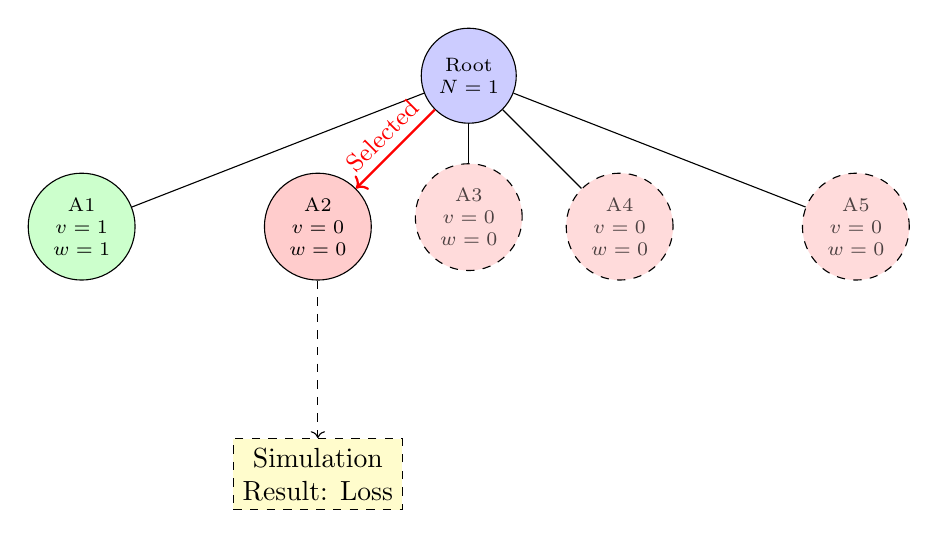
\begin{tikzpicture}[
    node distance=2.35cm,
    treenode/.style={circle, draw, minimum size=1cm, align=center, font=\scriptsize},
    root/.style={treenode, fill=blue!20, font=\scriptsize},
    unvisited/.style={treenode, fill=red!20, fill opacity=0.7, draw, dashed},
    selected/.style={treenode, fill=red!20},
    visited/.style={treenode, fill=green!20},
    simulation/.style={rectangle, draw, dashed, fill=yellow!20, align=center}
]

% Root node
\node[root] (root) {Root \\ $N=1$};

% Previous visited node
\node[visited, below left=1cm and 4cm of root] (a1) {A1 \\ $v=1$ \\ $w=1$};

% A2 is being expanded
\node[selected, below left=1cm and 1cm of root] (a2) {A2 \\ $v=0$ \\ $w=0$};
\node[unvisited, below=0.5cm of root] (a3) {A3 \\ $v=0$ \\ $w=0$};
\node[unvisited, below right=1cm and 1cm of root] (a4) {A4 \\ $v=0$ \\ $w=0$};
\node[unvisited, below right=1cm and 4cm of root] (a5) {A5 \\ $v=0$ \\ $w=0$};

% Simulation cluster
\node[simulation, below=2cm of a2] (sim2) {Simulation \\ Result: Loss};

% Edges and annotations
\draw (root) -- (a1);
\draw[->, thick, red] (root) -- node[above, sloped, font=\small] {Selected} (a2);
\draw (root) -- (a3);
\draw (root) -- (a4);
\draw (root) -- (a5);
\draw[dashed, ->] (a2) -- (sim2);

\end{tikzpicture}
\end{center}

\textbf{Backpropagation}: A2 loses $\Rightarrow$ $v=1$, $w=0$, Root $N=2$

\subsubsection*{Iteration 3: Third Expansion}

Select A3 (remaining unvisited node).

\begin{center}
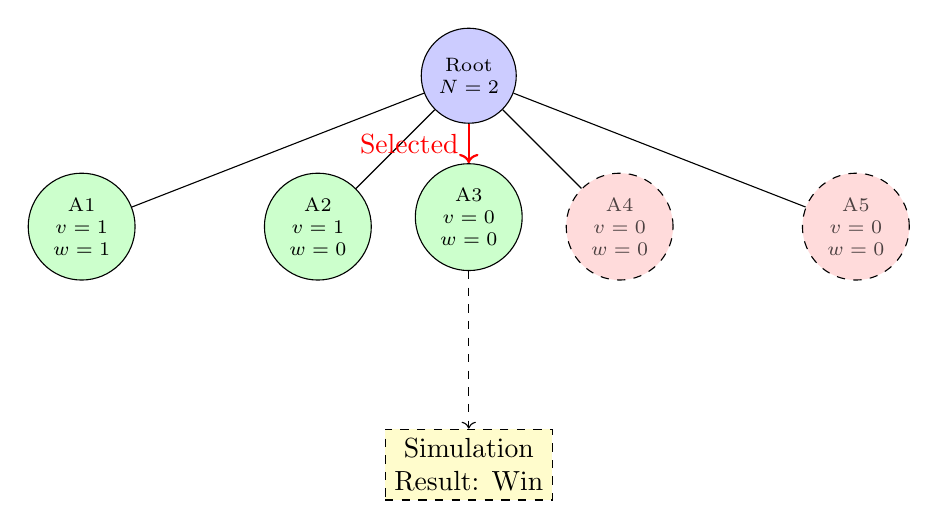
\begin{tikzpicture}[
    node distance=2.35cm,
    treenode/.style={circle, draw, minimum size=1cm, align=center, font=\scriptsize},
    root/.style={treenode, fill=blue!20, font=\scriptsize},
    unvisited/.style={treenode, fill=red!20, fill opacity=0.7, draw, dashed},
    visited/.style={treenode, fill=green!20},
    simulation/.style={rectangle, draw, dashed, fill=yellow!20, align=center}
]

% Root node
\node[root] (root) {Root \\ $N=2$};

% Previous visited nodes
\node[visited, below left=1cm and 4cm of root] (a1) {A1 \\ $v=1$ \\ $w=1$};
\node[visited, below left=1cm and 1cm of root] (a2) {A2 \\ $v=1$ \\ $w=0$};

% A3 is being expanded
\node[visited, below=0.5cm of root] (a3) {A3 \\ $v=0$ \\ $w=0$};
\node[unvisited, below right=1cm and 1cm of root] (a4) {A4 \\ $v=0$ \\ $w=0$};
\node[unvisited, below right=1cm and 4cm of root] (a5) {A5 \\ $v=0$ \\ $w=0$};

% Simulation cluster
\node[simulation, below=2cm of a3] (sim3) {Simulation \\ Result: Win};

% Edges and annotations
\draw (root) -- (a1);
\draw (root) -- (a2);
\draw[->, thick, red] (root) -- node[left] {Selected} (a3);
\draw (root) -- (a4);
\draw (root) -- (a5);
\draw[dashed, ->] (a3) -- (sim3);

\end{tikzpicture}
\end{center}

\textbf{Backpropagation}: A3 wins $\Rightarrow$ $v=1$, $w=1$, Root $N=3$

\subsubsection*{Iteration 4: Fourth Expansion}

Select A4 (remaining unvisited node).

\begin{center}
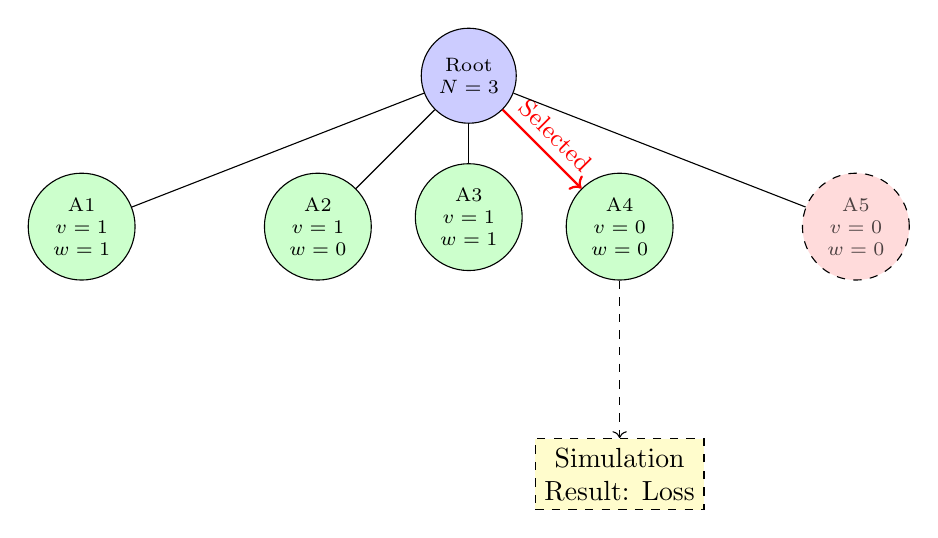
\begin{tikzpicture}[
    node distance=2.35cm,
    treenode/.style={circle, draw, minimum size=1cm, align=center, font=\scriptsize},
    root/.style={treenode, fill=blue!20, font=\scriptsize},
    unvisited/.style={treenode, fill=red!20, fill opacity=0.7, draw, dashed},
    visited/.style={treenode, fill=green!20},
    simulation/.style={rectangle, draw, dashed, fill=yellow!20, align=center}
]

% Root node
\node[root] (root) {Root \\ $N=3$};

% Previous visited nodes
\node[visited, below left=1cm and 4cm of root] (a1) {A1 \\ $v=1$ \\ $w=1$};
\node[visited, below left=1cm and 1cm of root] (a2) {A2 \\ $v=1$ \\ $w=0$};
\node[visited, below=0.5cm of root] (a3) {A3 \\ $v=1$ \\ $w=1$};

% A4 is being expanded
\node[visited, below right=1cm and 1cm of root] (a4) {A4 \\ $v=0$ \\ $w=0$};
\node[unvisited, below right=1cm and 4cm of root] (a5) {A5 \\ $v=0$ \\ $w=0$};

% Simulation cluster
\node[simulation, below=2cm of a4] (sim4) {Simulation \\ Result: Loss};

% Edges and annotations
\draw (root) -- (a1);
\draw (root) -- (a2);
\draw (root) -- (a3);
\draw[->, thick, red] (root) -- node[above, sloped, font=\small] {Selected} (a4);
\draw (root) -- (a5);
\draw[dashed, ->] (a4) -- (sim4);

\end{tikzpicture}
\end{center}

\textbf{Backpropagation}: A4 loses $\Rightarrow$ $v=1$, $w=0$, Root $N=4$

\subsubsection*{Iteration 5: Final Initial Expansion}

Select A5 (last unvisited node).

\begin{center}
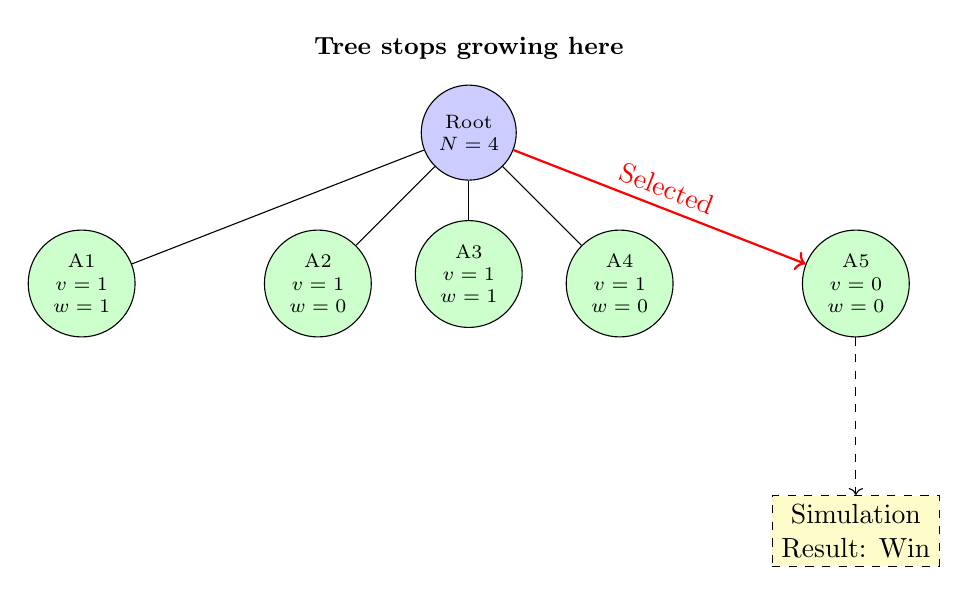
\begin{tikzpicture}[
    node distance=2.35cm,
    treenode/.style={circle, draw, minimum size=1cm, align=center, font=\scriptsize},
    root/.style={treenode, fill=blue!20, font=\scriptsize},
    unvisited/.style={treenode, fill=red!20, fill opacity=0.7, draw, dashed},
    visited/.style={treenode, fill=green!20},
    simulation/.style={rectangle, draw, dashed, fill=yellow!20, align=center}
]

% Root node
\node[root] (root) {Root \\ $N=4$};

% All nodes now visited
\node[visited, below left=1cm and 4cm of root] (a1) {A1 \\ $v=1$ \\ $w=1$};
\node[visited, below left=1cm and 1cm of root] (a2) {A2 \\ $v=1$ \\ $w=0$};
\node[visited, below=0.5cm of root] (a3) {A3 \\ $v=1$ \\ $w=1$};
\node[visited, below right=1cm and 1cm of root] (a4) {A4 \\ $v=1$ \\ $w=0$};

% A5 is being expanded (last one)
\node[visited, below right=1cm and 4cm of root] (a5) {A5 \\ $v=0$ \\ $w=0$};

% Simulation cluster
\node[simulation, below=2cm of a5] (sim5) {Simulation \\ Result: Win};

% Edges and annotations
\draw (root) -- (a1);
\draw (root) -- (a2);
\draw (root) -- (a3);
\draw (root) -- (a4);
\draw[->, thick, red] (root) -- node[above, sloped] {Selected} (a5);
\draw[dashed, ->] (a5) -- (sim5);

\node[above=0.2cm of root] {\small\textbf{Tree stops growing here}};

\end{tikzpicture}
\end{center}

\textbf{Backpropagation}: A5 wins $\Rightarrow$ $v=1$, $w=1$, Root $N=5$

\subsubsection*{Iteration 6: First UCB1 Selection}

Now all nodes have been visited. Calculate UCB1 ($c = \sqrt{2}$):

\begin{align*}
\text{UCB1}(A1) &= \frac{1}{1} + \sqrt{2} \sqrt{\frac{\ln 5}{1}} = 1 + 1.87 = 2.87 \\
\text{UCB1}(A2) &= \frac{0}{1} + \sqrt{2} \sqrt{\frac{\ln 5}{1}} = 0 + 1.87 = 1.87 \\
\text{UCB1}(A3) &= \frac{1}{1} + \sqrt{2} \sqrt{\frac{\ln 5}{1}} = 1 + 1.87 = 2.87 \\
\text{UCB1}(A4) &= \frac{0}{1} + \sqrt{2} \sqrt{\frac{\ln 5}{1}} = 0 + 1.87 = 1.87 \\
\text{UCB1}(A5) &= \frac{1}{1} + \sqrt{2} \sqrt{\frac{\ln 5}{1}} = 1 + 1.87 = 2.87
\end{align*}

Tie between A1, A3, A5. Randomly select A1.

\begin{center}
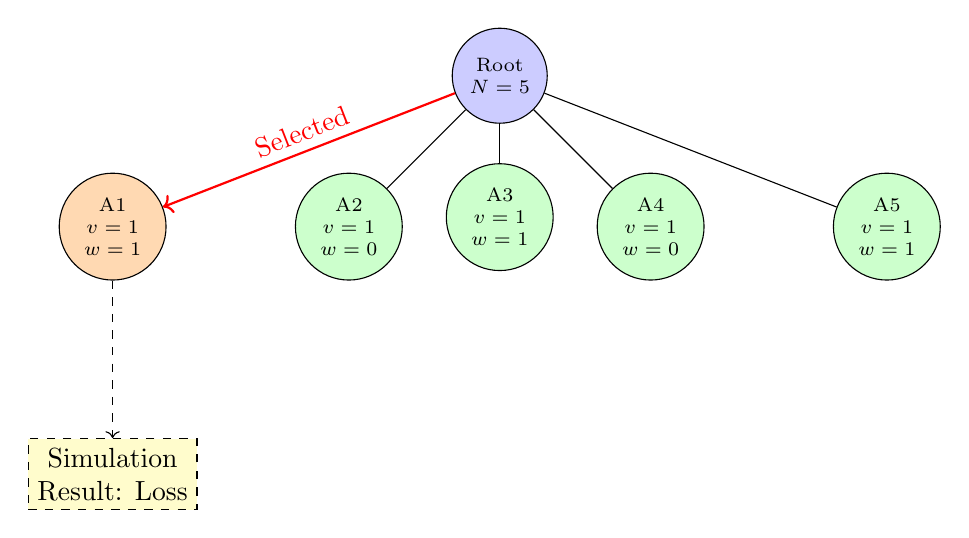
\begin{tikzpicture}[
    node distance=2.35cm,
    treenode/.style={circle, draw, minimum size=1cm, align=center, font=\scriptsize},
    root/.style={treenode, fill=blue!20, font=\scriptsize},
    visited/.style={treenode, fill=green!20},
    selected/.style={treenode, fill=orange!30},
    simulation/.style={rectangle, draw, dashed, fill=yellow!20, align=center}
]

% Root node
\node[root] (root) {Root \\ $N=5$};

% All nodes visited
\node[selected, below left=1cm and 4cm of root] (a1) {A1 \\ $v=1$ \\ $w=1$};
\node[visited, below left=1cm and 1cm of root] (a2) {A2 \\ $v=1$ \\ $w=0$};
\node[visited, below=0.5cm of root] (a3) {A3 \\ $v=1$ \\ $w=1$};
\node[visited, below right=1cm and 1cm of root] (a4) {A4 \\ $v=1$ \\ $w=0$};
\node[visited, below right=1cm and 4cm of root] (a5) {A5 \\ $v=1$ \\ $w=1$};

% Simulation cluster
\node[simulation, below=2cm of a1] (sim6) {Simulation \\ Result: Loss};

% Edges and annotations
\draw[->, thick, red] (root) -- node[above, sloped] {Selected} (a1);
\draw (root) -- (a2);
\draw (root) -- (a3);
\draw (root) -- (a4);
\draw (root) -- (a5);
\draw[dashed, ->] (a1) -- (sim6);

\end{tikzpicture}
\end{center}

\textbf{Backpropagation}: Only updates selected node $A_1$: $v=2$, $w=1$, Root $N=6$

\subsubsection*{Final Tree State}

After many iterations, the tree might look like:

\begin{center}
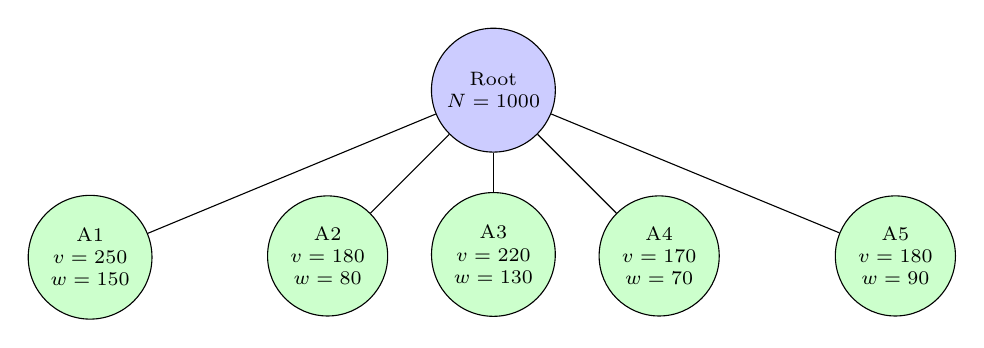
\begin{tikzpicture}[
    node distance=2.35cm,
    treenode/.style={circle, draw, minimum size=1cm, align=center, font=\scriptsize},
    root/.style={treenode, fill=blue!20, font=\scriptsize},
    visited/.style={treenode, fill=green!20, align=center}
]

% Root node
\node[root] (root) {Root \\ $N=1000$};

% Final statistics
\node[visited, below left=1cm and 4cm of root] (a1) {A1 \\ $v=250$ \\ $w=150$};
\node[visited, below left=1cm and 1cm of root] (a2) {A2 \\ $v=180$ \\ $w=80$};
\node[visited, below=0.5cm of root] (a3) {A3 \\ $v=220$ \\ $w=130$};
\node[visited, below right=1cm and 1cm of root] (a4) {A4 \\ $v=170$ \\ $w=70$};
\node[visited, below right=1cm and 4cm of root] (a5) {A5 \\ $v=180$ \\ $w=90$};

% Edges
\draw (root) -- (a1);
\draw (root) -- (a2);
\draw (root) -- (a3);
\draw (root) -- (a4);
\draw (root) -- (a5);

\end{tikzpicture}
\end{center}

\textbf{Final Decision}: Choose move with highest win rate\footnote{
    Or choose move with highest visit count
}: A1 ($150/250 = 60\%$)

\subsection*{When to Use Naive MCTS}

\begin{itemize}
    \item \textbf{Simple opponents}: When the opponent plays randomly or weakly
    \item \textbf{Computational constraints}: When deep lookahead is too expensive
    \item \textbf{Rapid prototyping}: Quick implementation for testing ideas
    \item \textbf{Very large branching factors}: When even one-ply exploration is challenging
\end{itemize}

\end{document}